\chapitre{Arnaque qui finit mal, le lundi 6 septembre 2027}{Depuis le matin,}{ Romain cueille ses cerises, rituel de fin d’été qu’il ne manquerait pas pour tout l’or du monde. Il en est ainsi depuis une bonne vingtaine d’années, depuis que ses douze cerisiers se sont mis à produire sérieusement, depuis qu’ils lui fournissent suffisamment de fruits pour que la Maririou fasse des tartes, des confitures, de la gelée, de l’eau-de-vie et pour que, tous les deux, ils en mangent durant des jours à pleine poignée. Comme de vrais enfants.}

L’aboiement des chiens est suivi d‘un bruit de moteur diesel et d’un crépitement de pneus sur la gravelle de l’entrée. Du haut de son escabeau, le septuagénaire se tourne et aperçoit une solide camionnette trois quarts de tonne qui s’immobilise près de sa galerie. Il reconnaît Jérôme Dubé, chemise western pistache (avec des cactus), blue-jean rétro, bottes de cowboy mordorées, Ray-Ban émeraude à monture sépia, qui claque la portière et qui se dirige vers la maison. Au même moment, la porte s’ouvre et Marie qui, de toute évidence, a entendu arriver le visiteur, l’accueille avec beaucoup plus d’entregent qu’elle n’en manifeste à son habitude.

- Jérôme ! Jérôme Dubé ! C’est pas croyable ! Un revenant !

- Un vrai revenant comme dans les films, Madame Rioux.

\begin{floatingfigure}[l]{40mm}
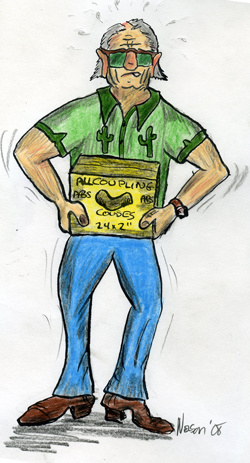
\includegraphics[height=60mm]{corps/chapitre5/img/jerome.jpg}
\end{floatingfigure}

Observant leurs effusions, Romain se souvient qu’à l’époque où Dubé travaillait avec lui comme assistant, la Maririou ne le détestait pas. Loin de là. N’eut été leur grande différence d’âge, elle se le serait peut-être offert. Mais encore eut-il fallut qu’elle soit plus chaleureuse qu’un frigo à bière. Malgré cela, allez savoir pourquoi, quand Romain amenait son jeune collègue à la maison, il fallait la voir se tordre le croupion comme une chatte en chaleur. Fantasme refoulé ?

Que peut donc lui vouloir ce petit malin à l’œil sournois, surtout que voilà bien neuf ans qu’il ne s’est pas pointé. Depuis la retraite du vieux camionneur.

- T’es-tu perdu, mon jeune ? qu’il lui fait en s’approchant.

- Rendu à mon âge, c’est toujours agréable de se faire traiter de «jeune» ! Comment ça va Romain ? Maudit que je suis content de te voir.

Il faudra une solide demi-heure de banalités avant que, cannette de bière en main, l’on passe au vif du sujet. Ce que voyant, Marie retourne à ses confitures en gardant, bien entendu, les deux oreilles grandes ouvertes. Ce qu’elle comprend, c’est que son beau Jérôme se cherche un chauffeur expérimenté pour un travail particulier et que c’est très payant. Extraordinairement payant.

- Je te parle de trois voyages non-stop, back-to-back, Sept-Îles – Toronto. Et au bout, il y a 150 000 \$ qui t’attendent.

Dans sa tête, la vieille dame traduit par «trois aller-retour collés», un périple sans doute fatigant, mais très bien payé. Et un périple probablement risqué. Sinon ça ne serait pas payé à ce tarif. Tout un montant. De quoi s’assurer une meilleure vieillesse. Mais encore faut-il que Romain accepte. Et rien n’indique qu’il va le faire.

- Je suis pas sûr que j’ai envie de rembarquer dans la gamique. C’est pour les jeunes, ça, pas pour un vieux comme moi. J’ai 75 ans et si je me fais attraper, je vais finir mes jours en prison. Ça ne me tente pas. J’ai encore de belles années devant moi, pas des masses, mais quelques-unes, et je n’ai pas envie de les perdre.

Dubé connaît assez Romain pour ne pas insister outre mesure.

- Je te donne mon numéro. Appelle-moi demain dans la journée pour me dire ce que tu décides. Si tu veux vraiment pas, je vais comprendre, mais va me falloir demander à un autre.

Et le gars de s’en retourner dans sa camionnette sous les aboiements.

- Vas-tu te taire, Gros-Prince, pis toi aussi Bedette !

Lorsque, deux heures plus tard, il commence à entrer quelques grands paniers de cerises pour entreprendre leur équeutage, sa conjointe des 47 dernières années l’attaque de front. Elle a toujours fonctionné ainsi, pour son plus grand bien et son plus grand malheur. Elle veut ces 150 000 \$. Et elle les aura, dut-elle conduire elle-même de Sept-Îles à Toronto. De plus, Jérôme est très gentil de «nous» offrir un tel cadeau. Il «nous» fait une fleur. Ça, sur «nos» vieux jours.

- Justement ! Ton Jérôme, je n’ai jamais vraiment pu le piffer. Il a des yeux de rat. Y est pas franc du col. J’ai jamais su ce qu’il pensait !

- Mais voyons ! C’est le meilleur garçon du monde ! Toujours prêt à rendre service !

Fantasme refoulé ?

Et ce fut ainsi jusqu’au lit conjugal. La seule chose qui ne fut pas dite, mais que les deux vieux comprenaient parfaitement bien, c’était que Romain était jaloux de Jérôme, qu’il lui en voulait pour les jeux de croupe de la Maririou. Tant et si bien qu’au matin, tandis qu’il trempait un quignon de pain de ménage dans de la confiture aux cerises fraîche de la veille, il déclara que la nuit avait porté conseil et qu’il téléphonerait à Dubé pour «ramasser le contrat». Marie avait gagné !

Dans un bar de Rimouski, Jérôme lui expliqua l’affaire. Au nord de Matamek, pas trop loin de la Moisie, un hydravion larguerait quelques contenants.

- Je te parle de 90 kilos de coke pure, toute bien paquetée en briques d’un kilo, une valeur de 9 millions sur le marché.

Lui, Jérôme, irait les chercher, ce qui n’était pas de la tarte, et amènerait le tout chez lui, à Sept-Îles, où il préparait trois caisses de 30 briques chacune. Ensuite, il chargerait sa propre camionnette de boîtes toutes semblables, des contenants de coudes en ABS utilisés en plomberie. Mais au travers, il en dissimulerait un plein de cocaïne, lequel serait marqué d’un petit X rouge. Une fois la livraison faite à Toronto, on recommencerait pour le deuxième, puis pour le troisième.

- Pourquoi rien qu’un à la fois, pourquoi trois voyages, pourquoi pas trois gars ?

Jérôme avait expliqué que ses employeurs ne voulaient pas courir de risque.

- Si tu te fais ramasser, ils ne vont perdre que le tiers de leur stock. Pis pourquoi pas trois chauffeurs avec trois camions ? Parce que moins y a de monde dans l’affaire, mieux c’est.

- Ouin ! Mais pourquoi ta camionnette personnelle ?

- Parce que de nos jours, avec les nouvelles plaques électroniques et les GPS, y a plus personne qui veut prendre la route avec un camion volé. On ne ferait pas deux kilomètres avant de se faire barrer le chemin par la police.

Les explications n’avaient pas entièrement convaincu Romain.

Mais pour le versement des 150 000 \$ promis, Jérôme s’était montré plus volubile et lui avait dévoilé la toute dernière technique de blanchiment d’argent. Même si, à cette époque, l’imminent réseau des CRG n’était pas encore en place, il était devenu normal qu’un retraité fasse session notariée de ses biens et devienne ainsi pensionnaire dans un centre d’hébergement privé ou parapublic. C’était selon sa capacité mensuelle de payer. D’où la combine.

Comme tous les bandits n’étaient pas assassinés à 25 ans dans un stationnement de Toronto et que certains atteignaient l’âge de la retraite, les criminels avaient imaginé offrir aux vieux malfrats, une rente annuelle variant entre cinq et vingt mille dollars, une rente tirée sur une banque antillaise. En échange, avait soutenu le verbomoteur Jérôme, ils devaient ne pas poser de question sur un compte qu’on y ouvrait à leur nom «pendant quelque temps». Un gros compte ! Ils devaient aussi signer, les yeux fermés, le testament qu’on leur avait préparé. Ainsi, quand une organisation structurait une opération où il faudrait gratifier des intervenants, elle déposait dans un des ces comptes, tout l’argent nécessaire au soutien logistique, de l’argent qui se retrouverait ainsi nettoyé. Une fois l’opération terminée, on faisait prendre sa retraite au prête-nom et on entreprenait de lui verser fidèlement tous les mois, sa petite rente. Fini les soucis !

- Ça veut dire, mon Romain, qu’il y a quelque part au Canada, un bonhomme qui va bientôt te désigner dans son testament comme étant son héritier pour un montant de 150 000 \$. Autrement dit, un mois ou deux après ta troisième livraison, pas plus, tu vas recevoir la copie légale d’un testament accompagné d’un chèque notarié de 150 000 \$, un beau chèque entièrement légal que tu vas pouvoir déposer dans ton compte.

Une histoire comme celle-là, ça ne s’inventait pas. De toute façon, Romain n’était pas né de la dernière pluie et il avait pris certaines précautions.

C’est ainsi que le lundi suivant, après une courte envolée Mont-Joli – Sept-Îles, Romain se présenta sur l’heure du midi chez son ancien assistant. Il se fit alors expliquer le trajet, le détail bien précis pour se rendre à l’entrepôt de Mississauga en banlieue de la Ville reine, ainsi que les noms des deux gars qui l’y recevraient.

- Y a une petite formalité avant que tu décolles, fit-il en ramassant un canif et une roulette de papier collant, viens avec moi.

La camionnette était stationnée devant la maison et Romain remarqua qu’elle avait la caisse arrière emplie de boîtes en carton identifiées à de la tuyauterie ABS. Son hôte lui fit signe de grimper avec lui et, en petit bonhomme sur le chargement, il déplaça deux boîtes pour être en mesure d’en soulever une troisième dont il coupa le scellant et ouvrit les deux rabats du dessus. Une fois le revêtement de plastique foncé dégagé, il fut possible d’entrevoir les briques du dessus.

- À c’t’heure, fouille dedans et sors en une au hasard. On va l’ouvrir et tu vas y tremper le bout de ton doigt pour y goûter. Comme ça, tu sauras ce que tu transportes.

- Si c’est de la mélamine à Chinois ?

- On verra bien ! Faut que tu saches ! Ils sont comme ça, mes clients !

Après s’être exécuté, Romain grimaça un début de sourire.

- Y a des goûts qui se perdent pas !

Le plus sérieusement du monde, le vieil homme sortit de sa poche un petit trousseau de clés sur lequel était accroché un cube noir de la taille d’un dé à jouer.

- Ça ramasse 600 mégapixels, c’est capable de capter un concert, ça se connecte partout, ça fait tout et ça coûte des pinottes. Là, ça va me servir à filmer la plus grosse quantité de poudre que j’ai jamais vue de ma vie ! J’ai hâte de montrer ça à Marie !

- Pas de danger de me voir la bette ?

- Non non, je ne prends que la boîte.

Une fois le souvenir capté, Jérôme referma le blanc pavée avec soin, le replaça, remit le plastique, recolla les deux battants et déposa les boîtes à leur place. Puis, les deux hommes revinrent sur le trottoir et, côte à côte, s’appuyèrent sur le côté de la caisse de la camionnette. On aurait dit deux copains parlant du dernier match de soccer.

- As-tu vu le X rouge sur la boîte ?

- Je l’ai photographié dans ma tête. Il est sur la boîte juste en dessous de celle-là.

- OK. Ça va aller ?

Devant le signe de tête de Romain, il lui tendit les clés du véhicule.

- Monsieur Romain !

C’était Josiane, la sculpturale conjointe de Jérôme qui l’appelait depuis la porte de côté, celle qui donnait sur la cuisine.

- Vous allez pas partir comme ça, venez manger quelque chose, c’est loin Toronto.

- Non merci, j’ai pas une grosse faim.

- Juste une petite pointe de tarte, alors ? Vous pouvez pas me refuser ça, elle est à la chicouté, c’est moi qui l’ai faite.

Le mot chicouté fut décisif.

- Ça fait de siècles que j’ai pas goûté à ça !

Quand le boulevard Laure recommença à s’appeler 138 à la sortie de Sept-Îles, Romain fit passer son moteur en mode électrique. Il n’avait jamais conduit de véhicule équipé d’un de ces nouveaux accumulateurs à haute performance et il ignorait jusqu’où il pourrait se rendre sur une même charge. Jérôme lui avait bien parlé de Tadoussac, une distance de plus de 400 kilomètres, mais il en doutait; il devrait probablement revenir au très onéreux mode diesel. Les faits lui donnèrent raison puisque l’accumulateur indiqua «Empty» un peu passé Forestville, à environ quatre-vingts kilomètres de sa destination.

Arrivé à Tadoussac en fin d’après-midi, il chercha un motel où il pourrait se louer une chambre, ce qui lui donnerait le droit de recharger son système de batterie. Malheureusement, tous les établissements hôteliers affichaient complet. On lui conseilla alors de continuer jusqu’à La Malbaie, 70 kilomètres de l’autre côté du fjord. C’est ainsi que le septuagénaire prit le traversier et fila vers la petite ville touristique.

Mais plus il roulait, plus le sentiment que quelque chose clochait grandissait en lui. Au départ, les explications au sujet des trois voyages ne l’avaient pas satisfait. Ensuite, si le 150 000 \$ promis étaient bien réels, pourquoi Jérôme, propriétaire de la camionnette, ne les faisait pas lui-même, ces voyages vers Mississauga ? Pour une telle somme, Romain aurait pu rouler jusqu’à la Terre de Feu! Puis, cette histoire de tarte à la chicouté le turlupinait. Voilà une belle fille, Josiane, à l’accent montréalais qui n’avait absolument rien d’une personne capable de préparer des tartes à la chicouté ou à n’importe quoi. Elle l’avait sûrement achetée, sa tarte, laquelle, de toute façon, goûtait la pâtisserie «achetée faite». Si tel était le cas, pourquoi avoir prétendu l’avoir faite elle-même ?

À La Malbaie, Romain aperçut un resto-pompe UltraTard, le fleuron local d’une chaîne de casse-croûte pas trop santé ouverts 24 heures, où il était possible de troquer ses batteries mortes contre des rechargées, de faire le plein en diesel ou, quand il y en avait, en essence ordinaire. Il s’approcha d’une pompe, inséra le pistolet et, même si son réservoir était loin d’être vide, commença son ravitaillement, les coudes appuyés sur la caisse arrière de la camionnette, ce qui lui permettait de voir tout son chargement. Il s’aperçut ainsi que les boîtes du dessus avaient glissé légèrement, ce qui laissait paraître, quelque peu, celles d’en dessous, incluant celle ornée d’un X rouge. C’est à ce moment qu’il eut la certitude d’avoir été floué. Appuyé sur la camionnette du côté conducteur, il n’aurait pas dû être capable de voir le X, lequel n’était visible que du côté passager, comme il avait pu constater en procédant aux vérifications à Sept-Îles. Ou bien on avait ajouté un deuxième X, ou bien la précieuse boîte avait été manipulée.

Le goût de la tarte à la chicouté lui revint !

- J’ai été eu !

Il grimpa dans la caisse, dégagea la boîte marquée et l’ouvrit. Elle ne contenait que de la poussière de pierre. C’est plus qu’il n’en fallait pour que son cerveau soit mis en mode «alerte rouge». Des malfaiteurs l’attendaient à Mississauga avec trente kilos de cocaïne. Or, il ne les avait plus. Cela parce qu’au moment où Josiane lui avait servi sa foutue pointe de tarte, Jérôme avait remplacé la boîte de coke par celle-ci.

Conclusion, Jérôme avait volé ses employeurs et il entendait lui faire porter le chapeau. Or, les méchants ne croiraient pas un seul mot de l’histoire que Romain leur raconterait, cela s’il était assez idiot pour continuer son périple jusqu’à Mississauga. Et, tant qu’à patauger dans la crosse, se pouvait-il que le salopard ait rapporté le vol de sa camionnette pour que les flics ne l’arrêtent ? Non, car il fallait qu’il roule jusqu’à Mississauga pour que les propriétaires de la poudre, des gens qui n’étaient sûrement pas dans un entrepôt de la Maple Leaf City, mais possiblement dans un bureau de la métropole québécoise, le croient coupable du vol.

Sans perdre un instant, il alla payer son diesel et conduisit son véhicule, comme si de rien n’était, vers le stationnement du terminus Intercar, deux coins de rue plus loin. Le tableau de bord étant muni de ressources téléphoniques, il fouina dans sa poche – il n’était pas bête – et il appela Jérôme.

- Y a un problème, lui dit-il d’entrée de jeu.

- Ah oui ?

- Tu m’as changé ma caisse de poudre pour une caisse bidon. J’arrête le contrat, p’is je descends à Sept-Îles te casser la gueule.

- Non non, fais pas ça. Faut vraiment que tu continues jusqu’à Toronto. Tu te trouves à agir comme leurre. Je n’ai pas le droit d’en parler, mais c’est comme ça. La bonne boîte de poudre est ailleurs. Mes employeurs craignent que les flics soient au courant et ils m’ont demandé d’arranger ça de même.

- Ah ouin ?

- Si tu te fais arrêter, ils trouveront rien et ils devront te relâcher. Par contre, pour les deux autres voyages, ça sera différent. Écoute faut que j’te laisse; j’ai ton «collègue» sur l’autre canal. Je te rappelle plus tard ! Bye !

Vraiment n’importe quoi ! Ce Jérôme Dubé le prenait pour un demeuré. Si ces détails étaient vrais, les donner, comme ça, au téléphone, relevait de la pire inconscience. Romain ramassa ses effets personnels, verrouilla la cabine et grimpa dans le dernier bus pour Québec, celui de 21h15, une nouveauté chez Intercar qu’affriandaient particulièrement les touristes gastronomes de la Vieille Capitale. Cependant, avant d’abandonner le camion, il se livra à une petite formalité, une minipolice d’assurance, au cas où !
Une fois à Québec, il prit le car de minuit 45 en direction de Rimouski et essaya de dormir.

Mais au même moment, Jérôme Dubé était sur le bord de la crise de nerfs.

Après sa petite manipulation pendant que Romain goûtait à la tarte de Josiane, il avait placé la boîte de 30 kilos, la seule et vraie boîte de cocaïne - les deux autres n’étant que billevesées imaginées pour mieux enfirouaper Romain - dans la section arrière de son automobile, une hybride trois portes très économique louée l’hiver dernier au moment où le prix du litre avait basculé à plus de 6 \$. Il savait pouvoir se rendre jusqu’à Tadoussac avec ses batteries chargées à bloc; il l’avait déjà fait. Au pire, il savait qu’il pourrait s’accommoder à Forestville; il connaissait un motel où il pourrait refaire sa charge tout en s’offrant une bonne nuit de sommeil.

De toute façon, il n’était pas pressé. Il avait tout son temps pour se présenter chez les deux Portugais près du parc Jeanne-Mance à Montréal, des gens qui ne semblaient pas craindre l’ire des vrais propriétaires de la coke, des hommes d’affaires au-dessus de tout soupçon qui avaient pignon sur rue à moins d’une heure de route plus au nord. Comme la qualité de son produit était excellente, le Septilien escomptait pouvoir en obtenir au moins un million et demi de dollars US versés dans un compte antillais ouvert à son nom.

À 16 h, il prenait la route, réalisant, au fur et à mesure qu’il les croisait, que toutes les stations d’essence n’avaient plus que du diesel. Mais, bon, il n’était pas inquiet, connaissant l’autonomie énergétique de son bolide. Le cœur en fête, il n’arrêta même pas à Baie-Comeau et traversa le pont de la Manic en rêvant de la dolce vita qui l’attendait dans les Caraïbes.

Pourtant, à quelques kilomètres de Ragueneau, la circulation commença à s’alourdir. Plus il approchait du village, moins il avançait. La 138 était bloquée. Jérôme se retrouvait prisonnier dans un convoi de véhicules long à ne plus finir, essentiellement des camions. De temps à autre, on avançait de quelques mètres. On aurait dit une meute affamée de gastéropodes flairant des laitues bien fraîches.

Il eut l’idée de syntoniser le canal d’urgence où il apprit que la 138 était temporairement fermée, un forcené s’étant barricadé dans sa maison avec des otages. On avait détourné la circulation dans un chemin de bois plus au nord, une route du siècle dernier qu’on n’avait pas conçue pour recevoir autant de fardiers. Tant et si bien que les plus lourds en arrachaient, peinaient et s’enlisaient. Rien n’allait plus.

C’est ainsi que Jérôme mit près de trois heures pour contourner le village en calant parfois jusqu’aux essieux. Eut-il dû faire volte-face et retourner à Baie-Comeau ? Oui, si on en croit les événements à venir. Car il s’aperçut que son système d’accumulation était presque épuisé. En fait, il ne lui restait même plus assez d’énergie pour atteindre Forestville, 50 kilomètres plus loin. Pire, le seul endroit où on aurait pu lui échanger ses batteries vides était fermé.

Mais la chance lui sourit au sortir du village quand il aperçut le placard tout illuminé du «Motel de la Forêt». Seul gîte du secteur, l’établissement semblait disposer de quelques bornes de chargement électrique non assignées. À l’officine d’accueil, un employé lui en désigna une tout près de la route, juste sous l’énorme enseigne. Jaugeant l’état général de délabrement du commerce, le voyageur préféra ne pas louer de chambre et s’en tenir au gavage de ses batteries. De toute façon, puisqu’une recharge complète ne prenait que deux heures avec les nouveaux accumulateurs, il calcula pouvoir reprendre la route à minuit et arriver à son hôtel de Tadoussac une heure plus tard. Ce qui n’était pas si mal.

Son auto branchée à la borne, Jérôme abaissa son dossier et s’écrasa confortablement en écoutant de la musique Motown. Au bout d’une demi-heure, la faim commença à l’incommoder; il n’avait rien mangé depuis le midi. Et encore ! Il n’avait avalé qu’une pointe de tarte à la chicouté accompagnée d’un verre de lait. Il eut l’idée d’aller à l’accueil se chercher des cochonneries, ce qui lui couperait la faim jusqu’à son arrivée à Tadoussac. Ce qu’il fit !

Malheureusement pour lui, deux paires d’yeux l’observaient depuis les fourrés. C’étaient deux jeunes Innus un peu paumés.

- Tshika ui shassikutshiakanu, tshe itinamuat mukumanu ushkutit. Tshek eka minupaniti, tshe tshitishimuiaku minashkuat, dit le plus vieux des deux, ce qui pourrait se traduire par : «On arrive à la course, tu lui pointes ton couteau sur le nez» (pour ne pas nuire à la compréhension du récit, nous allons continuer en français).

- Ouin.

- On l’oblige à sortir du char, on saute dedans et on se sauve. Ça marche ?

Le plus jeune n’avait pas l’air convaincu.

- D’in coup qu’i se défend ?

- On se pousse dans la nature !

- Ouin, j’sais pas …

- T’aimes-tu mieux marcher 25 kilomètres ? Moi pas !

Au même moment, Jérôme se glissa hors de sa voiture pour s’en aller à l’accueil.

- Attends, dit le plus vieux. Il s’en va au Motel. Es-tu capable de voir s’il a laissé ses clés ?

L’autre malvat s’approcha silencieusement et fit un signe affirmatif de la tête.

Cinq secondes plus tard, les deux gredins étaient assis dans la voiture, après l’avoir déharnachée de sa borne, et avaient mis le contact. Le plus vite qu’ils le purent, ils foncèrent sur la 138 et disparurent en direction de Betsiamites, une communauté établie en bordure du fleuve entre Ragueneau et Forestville.

Jérôme fut tellement ahuri par ce qu’il venait de voir que la bouche lui resta grande ouverte. Des gens venaient de fuir avec son million et demi de dollars US en belle poudre blanche ! Des gens qu’il ne connaissait pas, cela, le soir tard, dans un coin perdu où il n’avait aucun contact. L’employé du motel qui avait tout vu, accouru.

- Je les ai reconnus. Pas des méchants gars. D’habitude, ils font pas ça. Faut croire qu’ils étaient cassés. Ils s’en vont à Betsiamites avec ton char.

- Betsiamites, sur la Réserve ?

- C’est ça qu’i faut dire aux flics. Mais ça donnera rien. Comme d’habitude, ils vont attendre à demain et là, ils vont téléphoner à la police amérindienne. Surtout à soir; ils sont tous occupés avec le fou qui s’est barricadé. C’est sûr que ça va aller à demain. Et là, si ton char a pas été mis en morceaux, ils vont peut-être le trouver et te le ramener. Sinon, fais-en ton deuil !

Pour Jérôme, la cause fut vite entendue. Si les autorités retrouvaient l’auto dans les minutes suivant l’appel comme c’était souvent la pratique avec les technologies GPS, ils s’intéresseraient sûrement à la caisse de coudes en ABS marquée d’un X rouge. Ils sont comme ça, les flics. En revanche, s’ils n’entreprenaient les procédures que le demain, il est fort probable que les voleurs auraient ouvert la boîte et se seraient occupés de son contenu. Auquel cas, elle ne serait plus dans l’auto quand la police la retrouverait. Advenant qu’ils y arrivent, bien sûr. À ce moment, il n’y aurait plus de danger pour lui. Conclusion, il semblait plus prudent de rapporter le vol. Ce faisant, Jérôme se donnait même du temps pour fuir advenant qu’il doive le faire.

- J’ai plus rien pour téléphoner, c’était dans mon auto …

L’employé, un solide gaillard dans la trentaine, lui fit un signe de la main.

- Viens en dedans, on va t’arranger ça.

Dans la demi-heure qui suivit, Jérôme s’était fait aviser, tel que prévu, qu’en raison des événements, toutes les forces policières disponibles avaient été affectées au village et qu’ils communiqueraient, dès demain, avec leurs confrères de Betsiamites. Puis, la belle Josiane, la dame aux tartes achetées faites, lui avait promis qu’elle viendrait le prendre à Ragueneau, à l’autre bout du village, «pour ne pas être pognée dans le barrage routier», dans trois heures. En état de choc, ne pensant qu’à son million et demi et se sentant littéralement impuissant, l’ex-assistant de Romain Tardif dit le Gelé, avait accepté une bière de consolation et avait commencé à tuer le temps.

- Si j’y vas, là-bas, ça peux-tu donner des résultats ?

- Où, à Betsiamites ? À soir ?

- Oui

- Tu vas te faire casser la gueule. En plus de ne plus avoir de char, t’auras plus de dents.

- Je sais me défendre…

- Moi aussi, mais moi, je resterais ici bien tranquille.

Dubé n’avait pas été convaincu.

- Je te l’ai dit. Ce n’est pas du mauvais monde; ils vont probablement laisser ton char à un kilomètre de la réserve et finir à pied, ni vu ni connu. Ce sont pas des voleurs. Juste des jeunes sur le party.
Au même moment, les deux délinquants stationnaient la voiture devant une des maisons face à la plage. Assis sur sa galerie en train d’observer les reflets de la lune sur le fleuve, Joseph Picard les aperçut et leur fit signe. Depuis une dizaine d’années, l’homme était fortement impliqué dans une mécanique de redécouverte et de réappropriation de l’esprit innu, de la langue et des traditions, un long processus de redressement moral, de revalorisation sociale et de cheminement vers une fierté ethnique de bon aloi. Il questionna les deux gamins et quand il comprit, il ne put s’empêcher de les coiffer d’épithètes plutôt désagréables.

- Un Blanc qui vole un char, c’est rien, c’est juste un cave. Un Innu qui le fait, c’est un asti d’Indien. Pire, un Indien saoul ! Un Indien crotté ! Un Indien drogué ! C’est ça que vous voulez entendre quand la police va venir vous ramasser ?

Joseph s’approcha du véhicule et en fit le tour.

- C’est à qui ?

- À un Blanc qui s’était arrêté au premier motel à Ragueneau.

- C’est quoi la boîte en arrière ?

Les deux jeunes haussèrent les épaules.

Pris d’un doute, l’homme ouvrit le hayon et avec son couteau de poche, décacheta la boîte. Il ne lui fallut qu’un instant pour tout comprendre. Vivement, il fouilla dans ses poches, prit son trousseau de clés et le lança au plus vieux des deux noceurs.

- Toi, tu vas en arrière de la maison, tu ramasses un pic, une pelle et le cinq gallons d’essence sur la galerie, tu prends mon pick-up et tu me suis. Toi, le jeune, tu montes avec moi. Y a pas une minute à perdre.

- C’est quoi l’affaire ? demande celui-ci tandis que l’autre disparaît.

- L’affaire ? Vous vous êtes mis dans la marde. Le char que vous avez volé, il appartient à la grosse gamique. Tu veux-tu que son propriétaire à la boîte, il vienne ici la chercher ? Tu sais-tu ce qu’il y a dedans, la boîte ? Des kilos de coke ! C’te boîte-là, c’est la mort, la mort blanche, notre mort !

Cinq minutes plus tard, en plein bois, sur une route qu’on aurait dit conçue pour des VTT, l’auto électrique s’arrêta en panne sèche, façon de parler. Heureusement, Joseph avait une chaîne dans la caisse de sa camionnette. La voiture du Septilien Jérôme Dubé fut ainsi remorquée jusqu’à sa destination finale, un trou que les deux jeunes durent creuser, piquer, bêcher et pelleter pendant plus d’une heure, parce qu’il n’était pas assez creux. Ils y placèrent l’auto, Joseph l’enduisit d’essence et il l’enflamma. Puis, doucement, la tête vers le sol et les yeux fermés, il prit les mains tout endolories des deux malheureux.

- Ce qui brûle dans ce trou, c’est le mauvais en nous. Le mauvais qui sort, qui sort, qui s’en va dans les flammes. Dans le feu avec la mort blanche qui se brûle elle-même. Et le mauvais qui s’en va, il se trouve à laisser de la place, un vide. Un vide à côté du cœur, un vide à côté de l’esprit. Et un vide, ça peut pas rester vide. Faut que ça se remplisse. C’est la loi de la Terre. Et on a quoi pour le remplir le vide ? Seulement du bien, du bien qu’on va essayer de faire, du bien qu’on va générer, du bien qui appelle le bien, du bien pour nous, pour notre communauté, pour nos jeunes, nos aînés.

Dans la violence des flammes et de leur crépitement, un silence humain suivit.

- Bon, faut finir la job, à c’t heure ! finit par dire le mentor. Vous voyez le tas de roches ici à côté ?

- C’est des roches qui ont servi à des meteshun, fit le plus jeune, grand amateur de ces cérémonies de sudation spirituelle.

- C’est pas grave. Vous allez les placer sur l’auto pour bien la cacher. Faut que rien ne paraisse.
Personne ne devra savoir qu’en d’sour, y a un char et une boîte de mort au rat qu’on a fait brûler.

Il fallut encore une heure aux deux jeunes pour que le tas de pierres, des roches de la grosseur de gros pamplemousses, soit complètement déplacé sur la carcasse fumante. Au matin, les trois Innus revinrent avec des râteaux et quand ils eurent terminé leur nettoyage, plus rien de compromettant ne pouvait désormais attirer l’attention. De toute façon, d’ici l’hiver, la nature aurait parfaitement complété la dissimulation finale aussi bien d’une voiture neuve que d’une caisse terriblement létale.

Mais à Sept-Îles, Jérôme était sur le bord de la crise de nerfs.

Depuis son retour, vers 7 h, il tournait en rond, incapable de se concentrer sur la marche à suivre. Les ennuis s’accumulaient. À peine avait-il eu le temps d’arriver qu’un enquêteur de La Malbaie l’avait joint au téléphone. Il venait d’attraper les deux voyous qui avaient volé le chargement de coudes en ABS, un «chargement offert au grand jour» dans la caisse de la camionnette dont il était le propriétaire, un «véhicule oublié» au terminus d’autocars.

- Si vous pouviez passer d’ici 24 heures pour faire votre déposition et signer une pile haute comme ça se paperasse, ça ferait bien mon affaire.

- Oui, je m’en occupe.

- Juste comme ça, en passant. Pourquoi avez-vous laissé votre camionnette pleine de marchandise qui coûte cher, ici à La Malbaie ? Sur mon logiciel, je vois que vous êtes présentement à Sept-Îles. Vous êtes redescendu comment ?

Jérôme avait dû improviser rapidement.

- C’est une histoire de chicane avec ma conjointe. Elle est partie hier avec mon camion sur un coup de tête et, rendue à La Malbaie, elle a choisi de continuer en autobus.

- Une chicane d’amoureux.

- C’est ça.

- Votre conjointe a été filmée en train de faire le plein à l’UltraTard d’à côté et de descendre de votre véhicule au terminus d’autocars. Elle a même été filmée en train de s’acheter un billet pour la ville.

Le cœur de Jérôme avait cessé de battre.

- En venant faire votre déposition d’ici 24 heures, Monsieur Dubé, allez-vous avoir la gentillesse de m’expliquer pourquoi votre conjointe ressemble à un retraité à moustache portant une queue de cheval de l’ancien temps ? Et, tant qu’à me gratifier de vos bontés, allez-vous pouvoir m’expliquer le lien, si lien il y a, bien entendu, avec le vol de voiture que vous avez rapporté hier soir à Ragueneau ?

L’horreur n’avait plus de nom. Il ne lui restait plus d’autre choix que de filer et le plus tôt serait le mieux. Ainsi, Romain n’avait pas cru à son histoire de leurre et avait abandonné la camionnette à La Malbaie. Puis il avait pris l’autobus, probablement pour revenir chez lui. Ce n’était plus qu’une question d’heures avant qu’il ne rapplique ici avec un bâton de baseball.

- Sacrament !

Tout avait foiré. Les flics l’avaient dans leur collimateur, les Indiens avaient piqué la coke et Romain s’en venait lui casser la gueule. Il ne lui restait plus qu’une carte à jouer, ses «employeurs» du Nord de Montréal. Il leur dirait que le messager, un certain Romain Tardif que Josiane avait filmé en train d’inspecter son chargement et goûter à la poudre, laquelle on apercevait très bien sur le document, avait préféré livrer la marchandise aux Indiens de Betsiamites et qu’il était disparu avec l’argent. Il ajouterait que lui, Jérôme, il le recherchait partout et que s’il le trouvait, il lui ferait tout cracher. Comment il savait pour Betsiamites ? C’est que la puce de traçabilité placée dans la caisse avait cessé de fonctionner en plein milieu de la réserve.

Ce qu’il fit, en omettant toutefois de parler des Indiens et de Betsiamites, avant de se payer un aller simple sur le vol de l’après-midi Sept-îles-Montréal.

- C’est Josiane qui va être fâchée, dit-il en bouclant sa ceinture.

Au même moment, de l’autre côté du fleuve, Romain s’installait avec sa Maririou dans le chantier de Timothée sur la rue Crouet. À son arrivée à Saint-Anaclet, au petit matin, il était entré chez lui en criant au branle-bas de combat. Fallait se dépêcher, tout avait «chié», la combine n’était qu’une «crosse» pour que Jérôme fasse une «grosse passe», les «gars de la dope» avaient leur adresse ici à Saint-Anaclet, ils voudraient récupérer leur bien, ils étaient probablement déjà en route, il n’y avait plus une minute à perdre.

- Mais j’ai quand même une carte d’atout !

Romain le Gelé n’avait pas voulu en dire davantage. En une demi-heure, les deux vieux avaient empli leur voiture de tout ce qui, à leurs yeux, pouvait avoir de la valeur: papiers, partitions, instruments de musique, souvenirs, nourriture, quanticordi et un chiot laid comme les sept péchés capitaux que la Maririou appelait Gazou. Puis, ils avaient pris la poudre d’escampette. «La pédale au fond !» C’est la vieille qui appela Timothée pour qu’il les attende avant de partir pour son travail au ministère de la Santé. Mais c’est le bonhomme qui rappela pour annuler la consigne et pour, plutôt, lui donner rendez-vous dans un resto de Rimouski-Est.

Là, un plan d’action fut mis au point. On stationna d’abord l’automobile de Romain derrière l’édifice du ministère où Timothée officiait en tant qu’agent classe IV. Puis à coups de petits voyages discrets qui durèrent toute la journée, on transborda les effets personnels des deux vieux, lesquels dès le premier voyage, disparurent à tout jamais dans un sous-sol en pleine rénovation. Cet aspect du casse-tête réglé, Timothée abandonna la voiture de son père dans un rang sans surveillance sur les hauteurs de Rimouski et revint à pied. Il dut marcher pendant plus de trois heures.

Le lendemain matin, la télévision leur apprit que pendant la nuit, la fermette des Tardif, à Saint-Anaclet, avait été entièrement rasée par les flammes, un incendie probablement criminel, compte tenu de son extrême violence. Le corps des occupants, Romain Tardif et sa conjointe Marie Rioux, n’avaient pas été retrouvés dans les décombres, mais, fait navrant, les restes calcinés de deux grands chiens l’avaient été. Quant aux animaux de ferme, essentiellement de la volaille, quelques chèvres et des lapins, ils avaient tous été massacrés. Par ailleurs, la voiture du couple avait été retrouvée abandonnée sur le chemin d’un rang voisin. Enfin, disait-on, les enquêteurs étaient à la recherche de pistes et tout renseignement pouvant les aider était le bienvenu.

- Bedette, Gros Prince !

Romain avait pleuré, sans que la Maririou, le regard plus dur que jamais, n’arrive à lui mettre la main sur l’épaule.

Ainsi débuta la vie recluse du couple Tardif-Rioux. Pendant les premiers mois, les ajustements furent difficiles. Il fallut terminer les rénovations, cela sans revenus aucuns, l’État les considérant comme disparus ou décédés et leur compte en banque ayant été gelé par les autorités judiciaires. Il fallut également s’adapter à la promiscuité inhérente au petit logement du sous-sol. Mais le pire, c’est qu’il fallut se faire à l’idée que jamais plus ils ne pourraient aller profiter à leur goût du grand air.

\begin{floatingfigure}[l]{40mm}
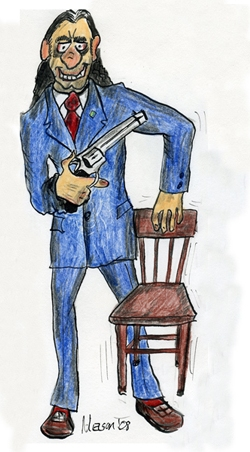
\includegraphics[height=60mm]{corps/chapitre5/img/alessandro.jpg}
\end{floatingfigure}

Le 8 février suivant, c’était un mardi en fin d’après-midi, le trio s’apprêtait à répéter une pièce, des pas se firent entendre dans l’escalier. Seul Gazou se montra hostile, prêt à l’attaque; les autres furent pétrifiés. Un homme habillé en président de compagnie et chaussé de pompes italiennes à 1 000 \$ pénétra dans la pièce et, d’un geste de la main, celle qui tenait le Smith \& Wesson modèle 500 à cartouches Magnum, fit comprendre à la Maririou qu’elle avait intérêt à policer sa bête.

- Gazou, ici, viens voir Maman !

À l’époque, elle n’avait pas encore commencé à chuinter.

Puis, de son canon, l’homme fit signe à Timothée de lui céder sa chaise.

- Je détesterais vous déranger trop longtemps, dit-il. Alors, je vais faire vite. Permettez-moi de me présenter, Alessandro Costi, homme de main. Mon travail, dans la vie, consiste à passer en arrière de crétins que mes clients utilisent bêtement quand ils veulent communiquer des messages. Moi, je ne mets jamais le feu et je n’égorge jamais de poules. Je me sers plutôt de ma tête. Par exemple, quand je cherche des gens qui n’ont pas laissé de traces et qui ne dépensent pas des fortunes dans des endroits extravagants, je regarde s’ils ont de la famille, ce qui est souvent facilité par les médias où on interview les enfants éplorés de parents dont les corps ont disparu. Et quand, de cette façon, je découvre un fils et que je m’aperçois qu’il achète de la bouffe pour trois, de la nourriture épouvantable, soit dit en passant, et du linge de femme dans des friperies, je me mets à suivre cet imbécile jusqu’à son terrier. Et là, bello caso, je descends les marches et devinez ce que je trouve ? Le type qui a été engagé pour livrer à mes clients trente kilos de coke mais qui a disparu avec la marchandise.

Personne n’osa parler. Seul Gazou eut le courage, ou la bêtise, de grogner.

- Comme personne ici n’a de temps à perdre, je vais poser la question une fois, une seule fois. Si, au bout de cinq secondes, je n’ai pas eu ma réponse, je tue le chien. Au bout de dix, je tue la madame et au bout de quinze, le fils à son papa, ici. Après, je vais devenir plus subtil. Mon pauvre monsieur, je vais devoir te faire éclater les rotules à coups de cartouches .500, ensuite les oreilles, puis quelques doigts et ainsi de suite, jusqu’à ce que j’aie ma réponse. Je ne pourrai malheureusement arrêter les tourments que si tu parles. Mais avant d’y arriver, si tu t’obstines, ça risque d’être assez long et pénible. Capito ? Alors voici la question : musique, roulements de tambour, gros plan sur le concurrent : où se trouvent les 30 kilos de poudre qui appartiennent à mes clients ?

Doucement, Romain déposa sa clarinette.

- C’est inutile. J’ai ta réponse. J’ai tout ça sur un mini cube numérique multifonction.

- Est-ce que ça nous apprend où est le bien de mes clients ?

- Non mais ça va b’en manque te montrer que je ne l’ai jamais eu et tu vas comprendre qui est parti avec.

Alessandro Costi réfléchit quelques instants.

- Perché no ? Je veux bien jouer le jeu; je ne suis pas à une minute près. Fais voir, mostrami !

Romain s’approcha d’un des rayons de bibliothèque et s’empara de l’édition 2006 du Petit Larousse qu’il ouvrit en son milieu. Un trou y avait été aménagé comme pour servir d’abri au mini-cube. Il le prit et le remit au visiteur.

- Ingegnoso ! Connecte-le à ton ordi, qu’on en profite tous ensemble.

Romain venait de jouer sa carte d’atout. Il avait enregistré l’intégralité de sa conversation avec Dubé dans un bar de Rimouski lorsque son ancien assistant lui avait expliqué le travail, incluant les trois livraisons à Toronto, le paiement de 150 000 \$ par chèque notarié et l’hydravion dans la région de Matamek. Puis ils purent visionner des images de la coke avec, comme fond sonore, les voix de Jérôme («Pas de danger de me voir la bette ?») et de Romain («Non non, je ne prends que la boîte»). Puis ce fut la conversation téléphonique où on lui révélait son rôle de leurre. Enfin, ce fut la scène du stationnement où on pouvait voir que la poudre avait été changée en poussière de pierre.

L’homme des choses interlopes se gratta le crâne avec le canon de son S\&W.

- Porca miseria ! Tu t’es fait boulechitter en grande, Signore Romano.

La Maririou regarda son vieux comme si c’était la première fois qu’elle le voyait, Timothée paru en phase de réanimation et Gazou déposa sa mauvaise tête sur ses petites pattes croches.

- Avec ces éléments nouveaux, il va se passer deux choses, mon bon Monsieur Romain. Moi, je m’en vais essayer de retrouver ton bon ami Jérôme. Amici dei miei amici sono miei amici, comme on dit à Ville-d’Anjou. Vois-tu, j’ai une question à lui poser. Une seule. Toi, Romano mio, tu vas rester ici bien tranquille avec ta femme et ton chien jusqu’à ce que je te fasse signe. Y a des cretinos dans la nature, ceux qui ont mis le feu et qui te cherchent encore. T’as compris ? Ne bouge pas, attend mon signal. Après, tu feras ce que tu veux. Pourquoi je vous élimine pas, toi et ta befana ? Parce que vous êtes trop vieux pour me nuire.

- Euh, et moi ?

- Toi le fils, fais comme d’habitude, mais sois prudent. Ils sont trop cons pour connaître ton existence. Dans ton cas, t’es p’t-être pas trop vieux pour me nuire, mais t’es trop timoroso. C’est ce qui te sauve la vie. On est bien peu de choses, non ? De toute façon, ça ne sera pas bien long avant que je vous fasse signe.

Exactement sept semaines plus tard, le 28 mars, Romain recevait un courriel 3D anonyme où on pointait sur un article de la Cyberpresse relatant la découverte d’un cadavre flottant sous le Pont de Québec. Jérôme Dubé avait été retrouvé.

- Tout un signal, s’était dit le vieil homme.

Mais la journée même, le Gros Turcotte déposait en chambre son projet de Réforme et en octobre suivant, un référendum faisait de Romain et Marie, deux illégaux. Auraient-ils pu, avant de le devenir officiellement, reprendre leurs identités et recommencer à bénéficier des services gouvernementaux ? Toucher des assurances ? Être dédommagés par le Fonds d’aide aux victimes d’activités criminelles ? Pour que cela soit possible, il leur aurait fallu expliquer une très longue histoire à différents corps de police, à différents bureaux de fonctionnaires, avec toutes les conséquences que cela aurait impliquées : procès, emprisonnement, danger de règlement de compte, peur constante, misère noire.

C’est probablement ce jour-là, le 28 mars 2028, qu’ils se résignèrent à finir leurs jours dans un sous-sol de Nazareth. Quant aux 30 kilos de cocaïne, ils ne furent jamais retrouvés. Par contre, Alessandro Costi, lui, il le fut vers la fin juin de la même année. Il marchait en chaussettes sur la 138, à mi-chemin entre Betsiamites et Forestville. Il était hagard. On l’avait dérouillé et dépouillé de sa voiture, de ses chaussures à 1 000 \$, de son Smith \& Wesson Magnum .500 et de son EP (émetteur personnel). Qui lui avait fait subir un tel traitement ? On ne le sut jamais. Par contre, il est permis de conclure qu’avant d’aller flotter sous le Pont de Québec, Jérôme Dubé avait pleurniché autour de l’histoire des deux jeunes de Betsiamites.